% Options for packages loaded elsewhere
% Options for packages loaded elsewhere
\PassOptionsToPackage{unicode}{hyperref}
\PassOptionsToPackage{hyphens}{url}
\PassOptionsToPackage{dvipsnames,svgnames,x11names}{xcolor}
%
\documentclass[
]{article}
\usepackage{xcolor}
\usepackage{amsmath,amssymb}
\setcounter{secnumdepth}{-\maxdimen} % remove section numbering
\usepackage{iftex}
\ifPDFTeX
  \usepackage[T1]{fontenc}
  \usepackage[utf8]{inputenc}
  \usepackage{textcomp} % provide euro and other symbols
\else % if luatex or xetex
  \usepackage{unicode-math} % this also loads fontspec
  \defaultfontfeatures{Scale=MatchLowercase}
  \defaultfontfeatures[\rmfamily]{Ligatures=TeX,Scale=1}
\fi
\usepackage{lmodern}
\ifPDFTeX\else
  % xetex/luatex font selection
\fi
% Use upquote if available, for straight quotes in verbatim environments
\IfFileExists{upquote.sty}{\usepackage{upquote}}{}
\IfFileExists{microtype.sty}{% use microtype if available
  \usepackage[]{microtype}
  \UseMicrotypeSet[protrusion]{basicmath} % disable protrusion for tt fonts
}{}
\makeatletter
\@ifundefined{KOMAClassName}{% if non-KOMA class
  \IfFileExists{parskip.sty}{%
    \usepackage{parskip}
  }{% else
    \setlength{\parindent}{0pt}
    \setlength{\parskip}{6pt plus 2pt minus 1pt}}
}{% if KOMA class
  \KOMAoptions{parskip=half}}
\makeatother
% Make \paragraph and \subparagraph free-standing
\makeatletter
\ifx\paragraph\undefined\else
  \let\oldparagraph\paragraph
  \renewcommand{\paragraph}{
    \@ifstar
      \xxxParagraphStar
      \xxxParagraphNoStar
  }
  \newcommand{\xxxParagraphStar}[1]{\oldparagraph*{#1}\mbox{}}
  \newcommand{\xxxParagraphNoStar}[1]{\oldparagraph{#1}\mbox{}}
\fi
\ifx\subparagraph\undefined\else
  \let\oldsubparagraph\subparagraph
  \renewcommand{\subparagraph}{
    \@ifstar
      \xxxSubParagraphStar
      \xxxSubParagraphNoStar
  }
  \newcommand{\xxxSubParagraphStar}[1]{\oldsubparagraph*{#1}\mbox{}}
  \newcommand{\xxxSubParagraphNoStar}[1]{\oldsubparagraph{#1}\mbox{}}
\fi
\makeatother


\usepackage{longtable,booktabs,array}
\newcounter{none} % for unnumbered tables
\usepackage{calc} % for calculating minipage widths
% Correct order of tables after \paragraph or \subparagraph
\usepackage{etoolbox}
\makeatletter
\patchcmd\longtable{\par}{\if@noskipsec\mbox{}\fi\par}{}{}
\makeatother
% Allow footnotes in longtable head/foot
\IfFileExists{footnotehyper.sty}{\usepackage{footnotehyper}}{\usepackage{footnote}}
\makesavenoteenv{longtable}
\usepackage{graphicx}
\makeatletter
\newsavebox\pandoc@box
\newcommand*\pandocbounded[1]{% scales image to fit in text height/width
  \sbox\pandoc@box{#1}%
  \Gscale@div\@tempa{\textheight}{\dimexpr\ht\pandoc@box+\dp\pandoc@box\relax}%
  \Gscale@div\@tempb{\linewidth}{\wd\pandoc@box}%
  \ifdim\@tempb\p@<\@tempa\p@\let\@tempa\@tempb\fi% select the smaller of both
  \ifdim\@tempa\p@<\p@\scalebox{\@tempa}{\usebox\pandoc@box}%
  \else\usebox{\pandoc@box}%
  \fi%
}
% Set default figure placement to htbp
\def\fps@figure{htbp}
\makeatother





\setlength{\emergencystretch}{3em} % prevent overfull lines

\providecommand{\tightlist}{%
  \setlength{\itemsep}{0pt}\setlength{\parskip}{0pt}}



 


\usepackage[scaled=.95]{cabin} 
\usepackage[varqu,varl]{inconsolata} 
\makeatletter
\@ifpackageloaded{tcolorbox}{}{\usepackage[skins,breakable]{tcolorbox}}
\@ifpackageloaded{fontawesome5}{}{\usepackage{fontawesome5}}
\definecolor{quarto-callout-color}{HTML}{909090}
\definecolor{quarto-callout-note-color}{HTML}{0758E5}
\definecolor{quarto-callout-important-color}{HTML}{CC1914}
\definecolor{quarto-callout-warning-color}{HTML}{EB9113}
\definecolor{quarto-callout-tip-color}{HTML}{00A047}
\definecolor{quarto-callout-caution-color}{HTML}{FC5300}
\definecolor{quarto-callout-color-frame}{HTML}{acacac}
\definecolor{quarto-callout-note-color-frame}{HTML}{4582ec}
\definecolor{quarto-callout-important-color-frame}{HTML}{d9534f}
\definecolor{quarto-callout-warning-color-frame}{HTML}{f0ad4e}
\definecolor{quarto-callout-tip-color-frame}{HTML}{02b875}
\definecolor{quarto-callout-caution-color-frame}{HTML}{fd7e14}
\makeatother
\makeatletter
\@ifpackageloaded{caption}{}{\usepackage{caption}}
\AtBeginDocument{%
\ifdefined\contentsname
  \renewcommand*\contentsname{Table of contents}
\else
  \newcommand\contentsname{Table of contents}
\fi
\ifdefined\listfigurename
  \renewcommand*\listfigurename{List of Figures}
\else
  \newcommand\listfigurename{List of Figures}
\fi
\ifdefined\listtablename
  \renewcommand*\listtablename{List of Tables}
\else
  \newcommand\listtablename{List of Tables}
\fi
\ifdefined\figurename
  \renewcommand*\figurename{Figure}
\else
  \newcommand\figurename{Figure}
\fi
\ifdefined\tablename
  \renewcommand*\tablename{Table}
\else
  \newcommand\tablename{Table}
\fi
}
\@ifpackageloaded{float}{}{\usepackage{float}}
\floatstyle{ruled}
\@ifundefined{c@chapter}{\newfloat{codelisting}{h}{lop}}{\newfloat{codelisting}{h}{lop}[chapter]}
\floatname{codelisting}{Listing}
\newcommand*\listoflistings{\listof{codelisting}{List of Listings}}
\makeatother
\makeatletter
\makeatother
\makeatletter
\@ifpackageloaded{caption}{}{\usepackage{caption}}
\@ifpackageloaded{subcaption}{}{\usepackage{subcaption}}
\makeatother
\newcounter{quartocalloutnteno}
\newcommand{\quartocalloutnte}[1]{\refstepcounter{quartocalloutnteno}\label{#1}}
\usepackage{bookmark}
\IfFileExists{xurl.sty}{\usepackage{xurl}}{} % add URL line breaks if available
\urlstyle{same}
\hypersetup{
  pdftitle={The Fermi-Pasta-Ulam-Tsingou problem},
  pdfauthor={Jacopo Tissino},
  colorlinks=true,
  linkcolor={blue},
  filecolor={Maroon},
  citecolor={Blue},
  urlcolor={Blue},
  pdfcreator={LaTeX via pandoc}}


\title{The Fermi-Pasta-Ulam-Tsingou problem}
\author{Jacopo Tissino}
\date{2026-06-09}
\begin{document}
\maketitle


\subsection{Motivation and history}\label{motivation-and-history}

The Fermi-Pasta-Ulam-Tsingou problem holds an important place in the
history of computational physics: it was first time a computer
simulation was used to obtain novel, interesting results about
fundamental physics.

From the evolution of a seemingly simple setup, a chain of oscillating
masses connected by non-linear springs, unexpected behaviour emerges.

This problem was studied in a 1953 paper, authored by Enrico Fermi, John
Pasta and Stanislaw Ulam. The paper included numerical simulations,
performed by Mary Tsingou who, instead of being credited as an author,
was simply
\href{https://web.archive.org/web/20240929141604/https://discover.lanl.gov/publications/national-security-science/2020-winter/we-thank-miss-mary-tsingou/}{mentioned
in a footnote}.

\subsection{Linear problem}\label{linear-problem}

\subsubsection{Description and ODE
approach}\label{description-and-ode-approach}

Consider a horizontal chain of masses connected by springs. Each of them
can oscillate in the vertical direction. We will use ``horizontal'' and
``vertical'' for clarity, but we are neglecting gravity here.

Hooke's law tells us that force is related to displacement through
\(\vec{F} = -k \vec{x}\); for the \(i\)-th mass, the horizontal
component of this force will always be balanced (since the horizontal
distance to its neighboring masses is fixed).

We can parameterize these masses through their vertical coordinates; the
\(i\)-th mass will be subject to a force

\[ F_i = -k (x_{i} - x_{i-i}) - k (x_{i} - x_{i+1})
= k ( x_{i-1} + x_{i+1} - 2 x_i )
\]

meaning that its acceleration, through \(F = m a\), will be

\[ \ddot{x}_i = \frac{k}{m} ( x_{i-1} + x_{i+1} - 2 x_i )\,.
\]

\begin{tcolorbox}[enhanced jigsaw, arc=.35mm, bottomrule=.15mm, bottomtitle=1mm, breakable, colback=white, colbacktitle=quarto-callout-note-color!10!white, colframe=quarto-callout-note-color-frame, coltitle=black, left=2mm, leftrule=.75mm, opacityback=0, opacitybacktitle=0.6, rightrule=.15mm, title=\textcolor{quarto-callout-note-color}{\faInfo}\hspace{0.5em}{Note \ref*{nte-title}: Physical constants}, titlerule=0mm, toprule=.15mm, toptitle=1mm]

\quartocalloutnte{nte-title} 

From here onward, we will set \(k/m = 1\) and forget about these
constants. Equivalently, we can work with a rescaled temporal coordinate

\[ \tilde{t} = t \sqrt{ \frac{m}{k}}\,.
\]

\end{tcolorbox}

\begin{tcolorbox}[enhanced jigsaw, arc=.35mm, bottomrule=.15mm, bottomtitle=1mm, breakable, colback=white, colbacktitle=quarto-callout-note-color!10!white, colframe=quarto-callout-note-color-frame, coltitle=black, left=2mm, leftrule=.75mm, opacityback=0, opacitybacktitle=0.6, rightrule=.15mm, title=\textcolor{quarto-callout-note-color}{\faInfo}\hspace{0.5em}{Note \ref*{nte-title}: Mass indices}, titlerule=0mm, toprule=.15mm, toptitle=1mm]

\quartocalloutnte{nte-title} 

We consider a system of \(N+1\) masses, indexed from \(0\) to \(N\),
such that masses \(0\) and \(N\) are kept fixed.

This means we have \(N\) springs, and the factor \(N\) will be used
often. Note that other references may say that \(N\) is the number of
masses.

\end{tcolorbox}

We expect wave-like solutions. Since we need to fix the boundaries to 0,
a sensible ansatz is

\[ x_i(t) = \sum_{n=1}^{N-1} Q_n(t) \sin\left( \frac{\pi i n}{N}\right)\,.
\]

Are these indeed solutions? Plugging them into our ODE we get

\[ \frac{\text{d}^2}{\text{d}t^2} x_i(t) = \sum_{n=1}^{N-1} \ddot{Q}_n(t) \sin\left( \frac{\pi i n}{N}\right) = (*)\,.
\]

On the other side, we have

\[ (*) = \sum_{n=1}^{N-1} Q_n(t) \left[ \sin\left( \frac{\pi (i+1) n}{N}\right) + \sin\left( \frac{\pi (i-1) n}{N}\right) - 2 \sin\left( \frac{\pi i n}{N}\right) \right]\,.
\]

Let us introduce the notation \(s_{x} = \sin ( \pi x / N)\) and
\(c_{x} = \cos ( \pi x / N)\), which will simplify the next step. We can
use the sine addition identity to write

\[ \sin\left( \frac{\pi (i \pm 1) n}{N}\right)
= s_{in} c_n \pm c_{in} s_n\,.
\]

Then, the RHS will equal

 
\begin{align}
(*) &= \sum_{n=1}^{N-1}
Q_n(t) \left[ 
    s_{in} c_n + c_{in} s_n 
    +
    s_{in} c_n - c_{in} s_n 
    - 2 s_{in}
 \right] \\
 &= \sum_{n=1}^{N-1} Q_n(t) s_{in} (2c_n - 2)\,.
\end{align}

and through another trigonometric identity we can get to

\[ 2 c_n - 2 = 2 (\cos \left( \frac{\pi n}{N}\right) - 1) = - 4 \sin^2 \left( \frac{\pi n}{2N}\right)\,.
\]

Then, if we denote \(\omega_n = 2 \sin (\pi n / 2N)\), we get to the
expression

\[ \sum_{n=1}^{N-1} \ddot{Q}_n (t) \sin\left( \frac{\pi i n}{N}\right) = -\sum_{n=1}^{N-1} \omega_n^2 Q_n(t) \sin\left( \frac{\pi i n}{N}\right)\,.
\]

Grouping the terms, we can write this as

\[ \sum_{n=1}^{N-1} \sin\left( \frac{\pi i n}{N}\right) \left[ \ddot{Q}_n (t) + \omega_n^2 Q_n(t) \right]  = 0\,.
\]

This should hold for all \(i = 0\dots N\) (for \(i=0\) and \(i=N\) those
equations are trivial since we always have \(x_i=x_N=0\)). We can
interpret this as a matrix equation: \(\sum_{n=1}^{N-1} U_{in}f_{n}=0\),
where \(U_{in} = \sin(\pi i n / N)\) while
\(f_{n} = \ddot{Q}_n (t) + \omega_n^2 Q_n(t)\). The matrix \(U\) is
invertible (check!), therefore the only solution to this system of
equations is \(f_{n}=0\) for all \(n\).

\subsubsection{Hamiltonian and matrix
approach}\label{hamiltonian-and-matrix-approach}

An alternative approach is the Hamiltonian one. We can write down the
Hamiltonian of the problem in terms of the momenta
\(p_{i} = \dot{x}_{i}\) and coordinates \(q_{i} = x_{i}\): \[
H = \frac{1}{2} \sum_{i=1}^{N-1} p_{i}^{2} + \frac{1}{2} \sum_{i=1}^{N} (x_{i} - x_{i-1})^{2}
\]

The equations of motion naturally appear from Hamilton's equations:

\begin{align}
-\frac{\partial H}{\partial x_{i}} &= -( x_{i}- x_{i-1} ) - (x_{i}-x_{i+1}) = x_{i-1} +x_{i+1} - 2 x_{i}  \\
\frac{\partial H}{\partial p_{i}} &= \dot{x}_{i}\,.
\end{align}

We can write the problem in matrix terms: the Hamiltonian will be \[
H = \frac{1}{2} \lvert \dot{x} \rvert ^{2} + \frac{1}{2} x^{T} V x\,,
\]

where \(V\) is a matrix with the following entries:

\begin{itemize}
\tightlist
\item
  \(2\) along the central diagonal, except for \(V_{00} = V_{NN} = 1\);
\item
  \(-1\) on the two diagonals near the central one.
\end{itemize}

\pandocbounded{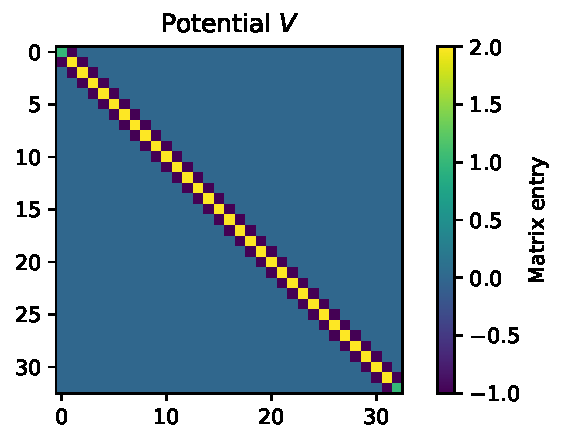
\includegraphics[keepaspectratio]{manuscript_files/figure-pdf/cell-5-output-1.pdf}}

We can diagonalize this potential making use of the matrix \(O\), whose
entries are given by \[
O_{nm} = \sqrt{ \frac{2}{N} } \sin\left(  \frac{nm\pi}{N} \right)\,.
\]

\(U\) is a symmetric, invertible matrix, and it is its own inverse:
\(OO = I_{N}\). The normalization \(\sqrt{2/N}\) is necessary in order
to achieve this.

A note of caution: the statement about invertibility is only true when
restricting the matrix to its central submatrix, with indices
\(1 \leq n, m < N\), since the outer ``cornice'' of the matrix is
identically zero, meaning that its rank is actually \(N-1\).

This transformation is called the \textbf{Discrete Sine Transform}, it
is a real-valued variant of the Fourier transform.

We can show that \(O^{T} V O = \Omega\), where \(\Omega\) is a diagonal
matrix.

\pandocbounded{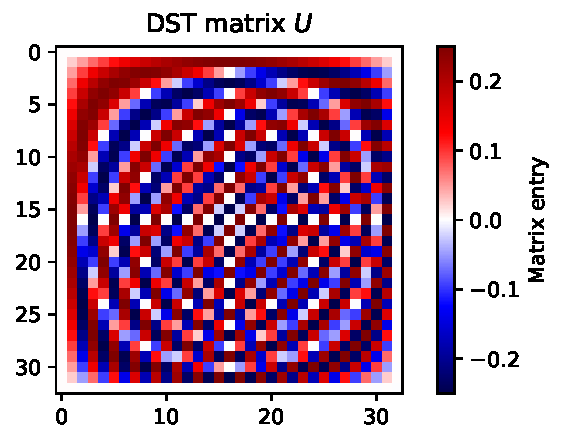
\includegraphics[keepaspectratio]{manuscript_files/figure-pdf/cell-6-output-1.pdf}}

\pandocbounded{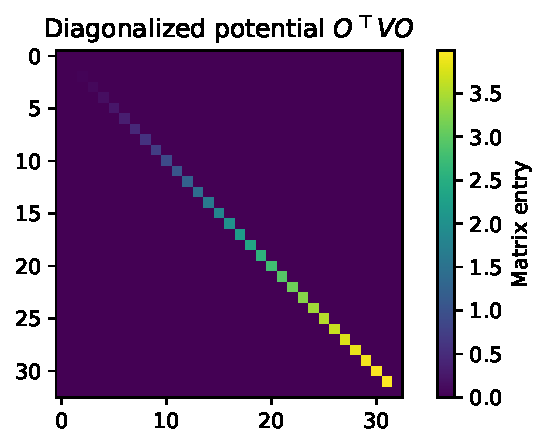
\includegraphics[keepaspectratio]{manuscript_files/figure-pdf/cell-7-output-1.pdf}}

Specifically, one finds that the entries on the diagonal of \(\Omega\)
are exactly the square angular frequencies from before:

\[ \Omega_{nn} = \omega_n^2 = 4 \sin^2 \left( \frac{\pi n}{ 2N} \right) \,.
\]

The coordinates \(Q\) can be written as \(Q = O x\), and they are called
\textbf{normal} coordinates. Since \(O\) is time-independent, we also
have \(\dot{Q} = O \dot{x}\). Since \(O\) is also its own inverse, we
also have \(x = O Q\) and \(\dot{x} = O \dot{Q}\).

In terms of these new coordinates, the Hamiltonian reads:

\[
H = \frac{1}{2} \sum_{n=1}^{N-1} \left[ \dot{Q}_{n}^{2} +\omega _{n}^{2}Q_{n}^{2} \right]\,,
\]

and it is natural to now consider the positions as \(q_n = Q_n\) and the
momenta as \(p_n = \dot{Q}_n\). From this formulation, it is clear that
each mode is evolving independently; not only is the \emph{global}
energy \(H\) conserved, but also each of its components

\[ E_n = \frac{1}{2}  \left[\dot{Q}_n^2 + \omega _{n}^{2}Q_{n}^{2} \right]
\]

is constant through the evolution. However, since each of the modes
evolves with a different frequency, their relative phases will change,
leading to a different shape for the \(x_i\).

\subsection{Non-linear problem}\label{non-linear-problem}

The linear problem is essentially solved. What is interesting is to see
how it changes when we introduce some nonlinearity; specifically, we
will make each spring react in a non-linear way,

\[
H = \frac{1}{2} \sum_{i=1}^{N-1} \dot{x}_{i}^{2} + \frac{1}{2} \sum_{i=1}^{N} \left[  (x_{i} - x_{i-1})^{2} + \frac{\alpha}{3}(x_{i}-x_{i-1})^{3} + \frac{\beta}{4} (x_{i}-x_{i-1})^{4}  \right]\,.
\]

\pandocbounded{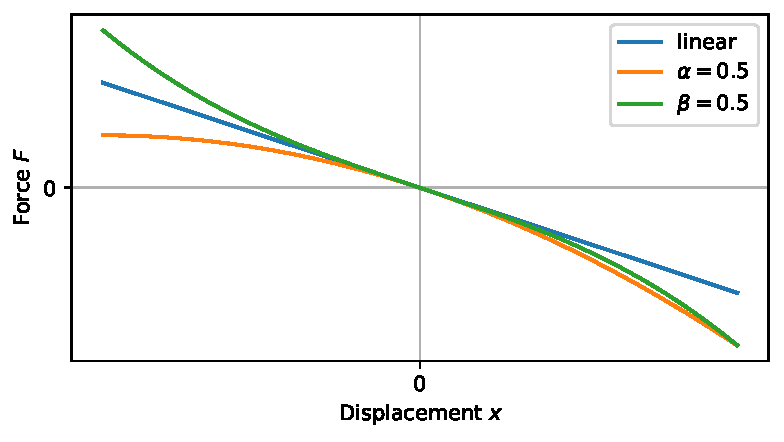
\includegraphics[keepaspectratio]{manuscript_files/figure-pdf/cell-8-output-1.pdf}}

The equations of motion now become \[
\ddot{x}_{i} = x_{i-1} +x_{i+1} - 2 x_{i} + \alpha \left[ (x_{i+1}-x_{i})^{2} - (x_{i}-x_{i-1})^{2} \right] + \beta \left[ (x_{i+1}-x_{i})^{3} - (x_{i}-x_{i-1})^{3} \right] \,.
\]

Now, the coordinates \(Q\) are not of particular help in \emph{solving}
the problem: the Hamiltonian written in terms of them remains heavily
coupled; for example, including only the \(\alpha\) contribution, we
have

\[
H = \frac{1}{2} \sum_{n=1}^{N-1} \left[\dot{Q}_{n}^{2} + \omega_n^2 Q_n^2\right] + \frac{\alpha}{3}
\sum{klm=1}^{N-1} c_{klm} Q_k Q_l Q_m \omega_k \omega_l \omega_m
\]

for some coeffficients \(c_{klm}\) which we do not need to actually
compute. This is not any easier to solve than the version written in
terms of \(x\); in fact, solving the equation in \(x\) is preferrable.

Nevertheless, understanding the linear problem is helpful when looking
at the evolution of the nonlinear one. We can still perform the
transformation \(Q (t) = Ox(t)\), and compute the energy in each
eigenmode of the linear problem, \(E_n(t)\). We do not expect these to
be constant as a function of time. The physicists in the 1953 paper
expected to observe some kind of thermalization, \emph{i.e.} the
energies contained in each mode would approach a stable configuration
with each mode having roughly equal energy.

Insted, they observed an interesting recurrence behaviour! After a long
time, almost all the energy appeared to return to the fundental \(n=1\)
mode.

\begin{figure}[H]

{\centering \pandocbounded{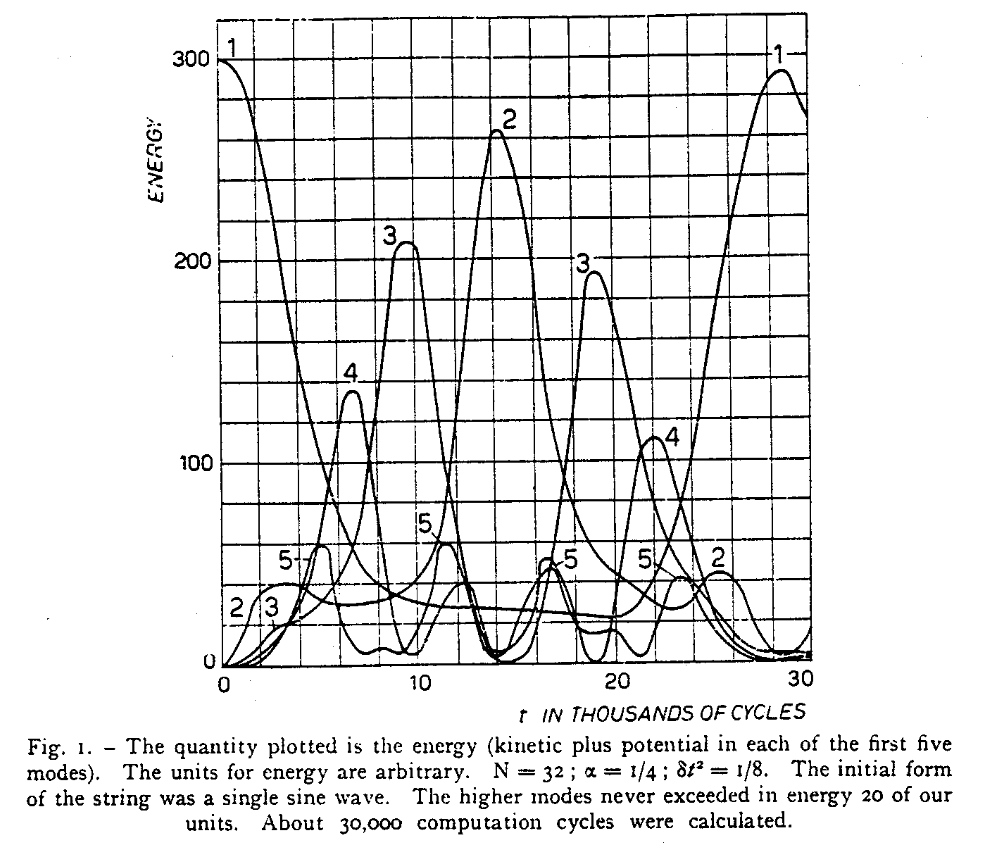
\includegraphics[keepaspectratio]{figure_1.png}}

}

\caption{Figure 1 from the 1953 FPUT paper.}

\end{figure}%

A lot of theoretical progress has been made since then, and the
recurrence time can be
\href{https://arxiv.org/pdf/nlin/0501053}{analytically estimated} as

\[ T_R = \frac{3}{\pi^{3/2} \sqrt{2}} \frac{N^{3/2}}{\sqrt{A \alpha}} T_1\,,
\]

where \(N\) is the number of springs, \(A\) is the initial amplitude of
the fundamental mode's oscillation, while \(T_1 = 2\pi / \omega_1\) is
the period of the fundamental oscillation.




\end{document}
